\subsection{Reaching definitions}
To solve our problem of detecting when unsanitized user input reaches a critical point in the code, we need an analysis of what assignments may influence the values of all variables at any point in the program.
The \emph{Reaching Definitions} as presented in \citet[p.~26]{schwartzbach} achieves just this.

Consider the Python code from the general example on \cref{theory:general_code_example}, repeated here, \cref{reaching::code}, so it is easier to follow.

\begin{lstlisting}[style=python, caption={General code example repeated here from \cref{theory:general_code_example}}, label=reaching::code]
x = input()
x = int(x)
while x > 1:
    y = x / 2
    if y > 3:
        x = x-y
    z = x-4
    if z > 0:
        x = x / 2
    z = z - 1
print(x)
\end{lstlisting}

The code is very simple, it take some user input which is sent through a while loop that changes the three variables x,y and z.
The x variable is printed out as the last operation of the program.
At this point x has been changed by assignments a number of times, and it is not obvious where the value comes from.
By performing the reaching definitions analysis we can find possible origins of the value.

\paragraph{Performing the analysis}
As stated earlier a dataflow analysis consist of many of the concepts that have been introduced until now.
These concepts will in the following be instantiated on the previously introduced example as to present the complete analysis.

\subparagraph{Control flow graph}
The CFG of this code is presented in \cref{reaching::cfg}.

\begin{figure}
  \begin{center}
  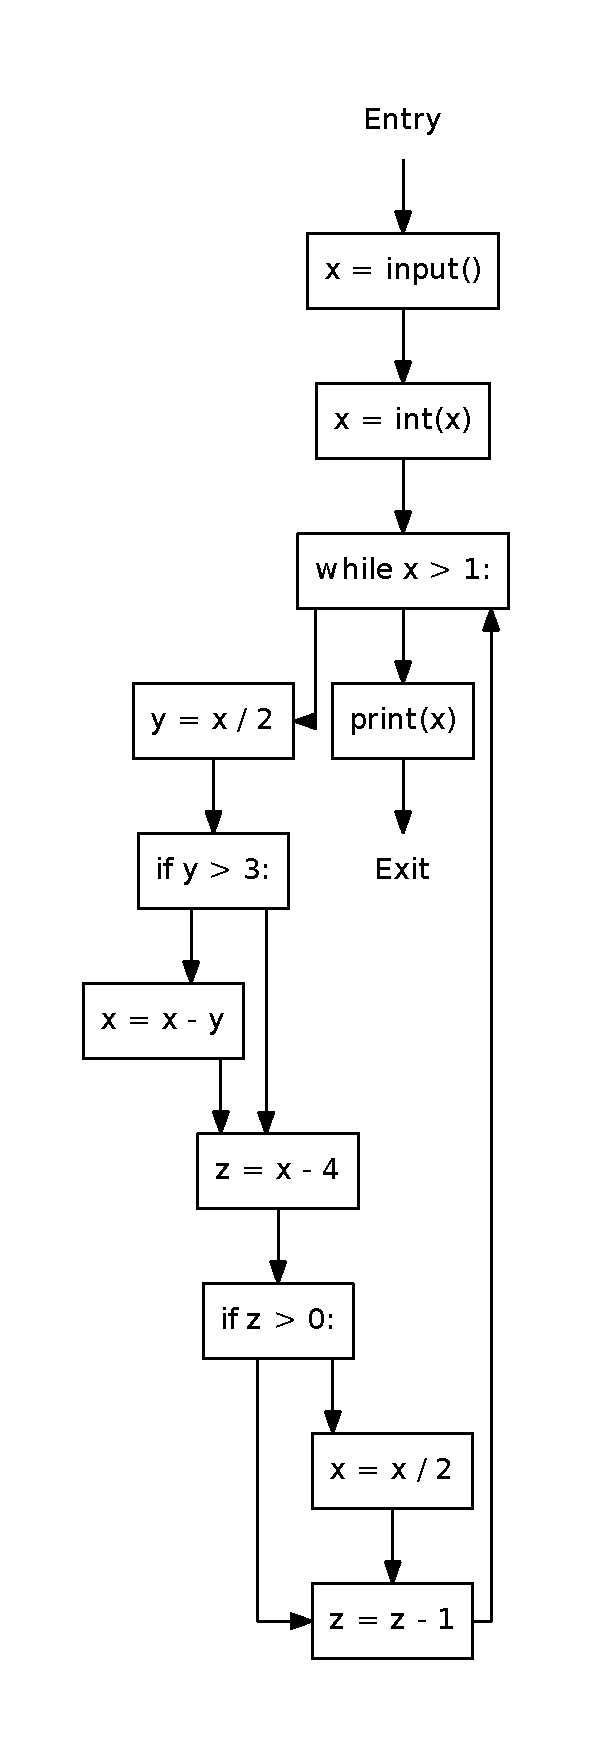
\includegraphics[scale=.5]{./figures/reaching_definitions.pdf}
  \caption{CFG of the python code presented in \cref{reaching::code}}
  \label{reaching::cfg}
  \end{center}
\end{figure}

The flow is linear until the while loop.
The while loop diverts the flow into the loop and ultimately to the print statement.
The loop has two if statements where the flow is again split up.
It is easy to see from the flow graph that there are many possible routes from entry to exit, and the propagation of values is not straightforward.

\subparagraph{Lattice}
The lattice used for this analysis is a power set lattice of all the assignments in the program.

\[ L = ( 2^{ \{x = \text{input()}, ~ x = \text{int(x)}, ~ y = x/2, ~ x = x-y, ~ z = x-4, ~ x = x/2, ~ z = z-1 \} } , \subseteq ) \]

\todo{visualisation of the lattice - do this or not?}

\subparagraph{Dataflow Constraint System}
The analysis is performed backwards by joining the constraints of all predecessors of all nodes.
This can be expressed a the following function:

\[ JOIN(v) = \bigcup_{ w \in pred(v)} \constraint{w} \]

All nodes other that assignment just join all constraints of their predecessors:

\[ \constraint{v} = JOIN(v) \]

Assignment nodes changes the content of a variable and the former assignment to this variable will therefore be discarded:

\[ \constraint{v} = JOIN(v) \downarrow id \cup \{ v \} \]

Where the $\downarrow$ function removes all assignments to the variable $id$ from the result of the JOIN.

Applying the previously defined dataflow constraints to the generated CFG looks as follows:

\begin{figure}[H]
\[
\begin{array}{lcl}
  \constraint{entry} & = & \{\}\\
  \constraint{x = input()} & = & \assignconstraint{\constraint{entry}}{x}{x = input()}\\
  \constraint{x = int(x)} & = & \assignconstraint{\constraint{x = input}}{x}{x = int(x)}\\
  \constraint{\text{while } x > 1} & = & \constraint{x = int(x)} ~ \cup ~ \constraint{z = z - 1}\\
  \constraint{ y = x / 2} & = & \assignconstraint{\constraint{\text{while } x > 1}}{y}{y = x / 2}\\
  \constraint{\text{if } y > 3} & = & \constraint{ y = x / 2}\\
  \constraint{ x = x-y} & = & \assignconstraint{\constraint{\text{if } y > 3}}{x}{x = x-y}\\
  \constraint{ z = x-4} & = & \assignconstraint{(\constraint{x = x-y} ~ \cup ~ \constraint{\text{if } y > 3})}{z}{z = x-4}\\
  \constraint{\text{if } z > 0} & = & \constraint{z = x - 4}\\
  \constraint{x = x / 2} & = & \assignconstraint{\constraint{\text{if } z > 0}}{x}{x = x/2}\\
  \constraint{z = z - 1} & = & \assignconstraint{(\constraint{\text{if } z > 0} ~ \cup ~ \constraint{x = x / 2}}{z}{z = z - 1}\\
  \constraint{print(x)} & = & \constraint{\text{while } x > 1}\\
  \constraint{exit} & = & \constraint{print(x)}
\end{array}
\]
\caption{Dataflow constraints applied on the generated CFG}
\end{figure}

\paragraph{Solving the equation system}
Solving this system of equations with the fixed-point algorithm will provide the information we need in order work with our problem.

The first iteration of this looks as follows:

\begin{figure}[H]
\[
\begin{array}{lcl}
  \constraint{entry} & = & \{\}\\
  \constraint{x = input()} & = & \{x = input()\}\\
  \constraint{x = int(x)} & = & \{x = int(x)\}\\
  \constraint{\text{while } x > 1} & = & \{\}\\
  \constraint{ y = x / 2} & = & \{ y = x / 2\}\\
  \constraint{\text{if } y > 3} & = & \{\}\\
  \constraint{ x = x-y} & = & \{ x = x - y \} \\
  \constraint{ z = x-4} & = & \{z = x-4 \} \\
  \constraint{\text{if } z > 0} & = & \{\}\\
  \constraint{x = x / 2} & = & \{ x = x / 2 \}\\
  \constraint{z = z - 1} & = & \{ z = z -1 \} \\
  \constraint{print(x)} & = & \{\}\\
  \constraint{exit} & = & \{\}\\
\end{array}
\]
\caption{First iteration of the fixed-point algorithm}
\label{reachingdefinitions:firstiteration}
\end{figure}

Here it is clear that only the constraints of assignments have walked up the lattice, each to the node indicating the flownode itself.
After nine iterations all the assignments will propagate through the program, and the result can be seen on \cref{reachingdefinitions:finaliteration}.
These constraints can now be interpreted in order to answer question that require knowledge of which assignments reach which nodes.

\begin{figure}[H]
\[
\begin{array}{lcl}
  \constraint{entry} & = & \{\}\\
  \constraint{x = input()} & = & \{x = input()\}\\
  \constraint{x = int(x)} & = & \{x = int(x)\}\\
  \constraint{\text{while } x > 1} & = & \{ x = int(x), ~ y = x / 2, ~ x=x-y, ~ x = x/2, ~ z=z-1 \}\\
  \constraint{ y = x / 2} & = & \{ x = int(x), ~ y = x / 2, ~ x=x-y, ~ x = x/2, ~ z=z-1 \}\\
  \constraint{\text{if } y > 3} &  = & \{ x = int(x), ~ y = x / 2, ~ x=x-y, ~ x = x/2, ~ z=z-1 \}\\
  \constraint{ x = x-y} & = & \{ y = x / 2, ~ x=x-y, ~ z=z-1 \}\\
  \constraint{ z = x-4} & = & \{ x = int(x), ~ y = x / 2, ~ x=x-y, ~ z=x-4, ~ x = x/2\}\\
  \constraint{\text{if } z > 0} & = & \{ x = int(x), ~ y = x / 2, ~ x=x-y, ~ z=x-4, ~ x = x/2\}\\
  \constraint{x = x / 2} & = & \{ y = x / 2, ~ z=x-4, ~ x = x/2\}\\
  \constraint{z = z - 1} & = & \{ x = int(x), ~ y = x / 2, ~ x=x-y, ~ x = x/2, ~ z=z-1 \}\\
  \constraint{print(x)} & = & \{ x = int(x), ~ y = x / 2, ~ x=x-y, ~ x = x/2, ~ z=z-1 \}\\
  \constraint{exit} & = & \{ x = int(x), ~ y = x / 2, ~ x=x-y, ~ x = x/2, ~ z=z-1 \}\\
\end{array}
\]
\caption{Final result of the fixed-point algorithm}
\label{reachingdefinitions:finaliteration}
\end{figure}

\paragraph{Interpreting the result}

Looking at the final equations the potential flow of values through the program can be seen.
For example, looking at the print statement, the value of x could have originated from three places in the program: the $x = int(x)$, $x = x-y$ or the $x = x/2$ statement.
Depending on the purpose of the analysis, this information can be used to deduce whether any dangerous flows are possible.
